\subsection{Evaluation sets} \label{eval_datasets}

Subject assignments can be evaluated with the metadata of the documents. \cite{toepfer2020fusion} mentions this possibility, stating that they plan on developing an automatic quality estimation metric that is based on meta information of the documents. For example, documents that are published in the same journal can be expected to be semantically similar. The publisher clearly delimits the field to which the publication belongs to. Our approach, although it also uses the metadata to evaluate the methods, is more straight forward. We extract subjects and venues (including referees and advisors of theses) from the repositories to construct three evaluation sets.

The first evaluation set comprises the handwritten subjects of the repositories, i.e. those that the users input manually when uploading a new document. We have mapped our complete set of subjects to the handwritten subjects of the repositories with a string matching procedure. Doing so, we could create an evaluation set with over 9,000 assignments. This evaluation set is the only one that considers further subjects, other than fields.

\acrshort{ddc} subjects can also be used in this regard. They appear consistently throughout all three repositories, as shown in section \ref{subjects_ddc}, and don't suffer from potential duplicates that arise from the free-text input, as handwritten subjects do. We have manually mapped \acrshort{ddc} numbers to \acrshort{mag} fields of study, to construct our second evaluation set.

Using unsupervised methods to evaluate the set of subjects of theses may prove more challenging, as they are not published anywhere and their authors usually just have that one document in the repositories. Advisors and referees may be of use in this regard. Two theses advised by the same professor should be more similar than two theses advised by different professors. This is the same logic we followed in the \acrfull{um}. We create our third evaluation set by manually mapping venues, advisors and referees to \acrshort{mag} fields of study.

\subsubsection{Handwritten subjects} \label{eval_subjects}

We have mapped our subset of \acrshort{mag} subjects to those of the repositories, which were input manually by the users that uploaded the documents, hence the term ``handwritten subjects''. To increase the number of matches, we have done so in a case-insensitive manner, i.e. we have first lower-cased all subjects. This simple matching procedure yielded 1,272 subjects, meaning that 59 \% of our \acrshort{mag} subset is present in the repositories. The total number of assignments of subjects to documents is 9,052.

The most popular subjects are \textit{Climate change}, which is assigned to 154 documents, \textit{Sustainability}, with 124 assignments, \textit{Mass spectrometry}, with 87 assignments and \textit{Molecular dynamics}, with 76 assignments. Figure \ref{fig:docs_per_subject} shows how often each subject occurs in the repositories. 301 subjects are assigned to only one document, whereas 307 subjects are assigned to at least nine documents. On average, the subjects are assigned to seven documents of the repositories.

\begin{figure}
  \begin{subfigure}[t]{0.45\textwidth}
    \centering
    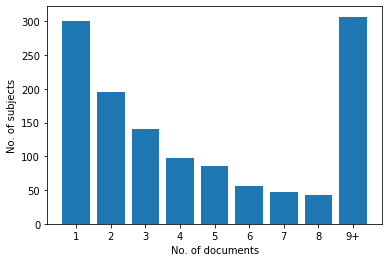
\includegraphics[width=\textwidth]{figures/evaluation/docs_per_subject.png}
    \caption{Handwritten subjects.}
    \label{fig:docs_per_subject}
  \end{subfigure}
  \hfill
  \begin{subfigure}[t]{0.45\textwidth}
    \centering
    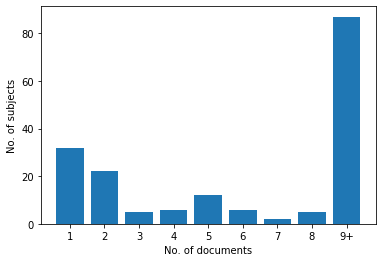
\includegraphics[width=\textwidth]{figures/evaluation/docs_per_ddc.png}
    \caption{DDC subjects.}
    \label{fig:docs_per_ddc}
  \end{subfigure}
  \caption{Distribution of the number of documents each subject (handwritten or DDC) is assigned to.}
\end{figure}

Another positive aspect of these subject matches is how well distributed they are across the fields. As can be seen in figure \ref{fig:eval_hw_fields}, all fields have assignments. \textit{Environmental science} is the least populated field, with 41 assignments. On the other hand, \textit{Medicine}, \textit{Biology} and \textit{Physics} have more than 200 assignments each.

\begin{figure}
  \begin{subfigure}[t]{\textwidth}
    \centering
    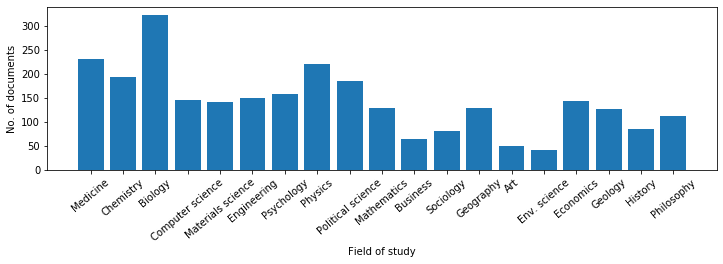
\includegraphics[width=\textwidth]{figures/evaluation/eval_hw_fields.png}
    \caption{Handwritten subjects}
    \label{fig:eval_hw_fields}
  \end{subfigure}
  \hfill
  \begin{subfigure}[t]{\textwidth}
    \centering
    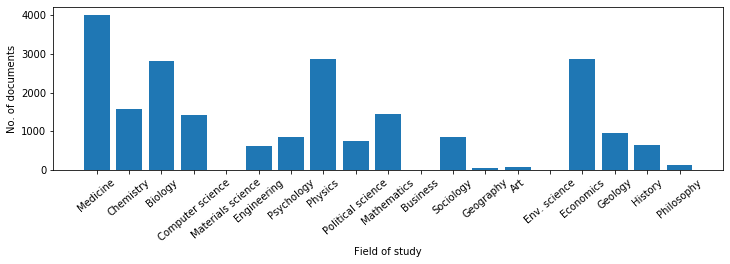
\includegraphics[width=\textwidth]{figures/evaluation/eval_ddc_fields.png}
    \caption{DDC subjects}
    \label{fig:eval_ddc_fields}
  \end{subfigure}
  \begin{subfigure}[t]{\textwidth}
    \centering
    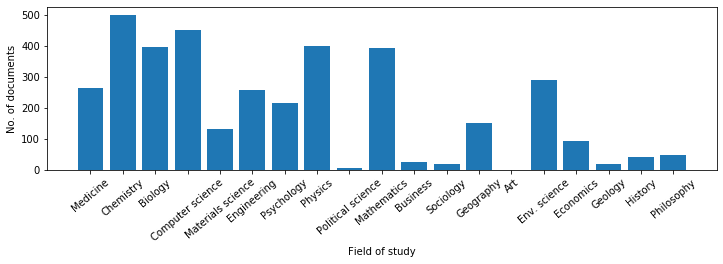
\includegraphics[width=\textwidth]{figures/evaluation/eval_venue_fields.png}
    \caption{Venues}
    \label{fig:eval_venue_fields}
  \end{subfigure}
  \caption{Number of assignments per field of study for handwritten subjects, DDC subjects and venues.}
\end{figure}

This evaluation set comprises 7,145 distinct documents. 78 \% of them only have one of the \acrshort{mag} subjects assigned to them, as shown in figure \ref{fig:eval_hw_fields}. On average, documents are assigned 1.27 subjects. Only one document has more than six assignments. It belongs to edoc and its subjects include \textit{Sustainability}, \textit{Climate change} and \textit{Poverty}, among others. Then there are two documents of refubium with six assignments, one about public law and the other about magnesium, potassium and other chemical elements.

The documents are also evenly distributed across repositories. Refubium has the largest amount of documents in this evaluation set, with 3,208. This makes sense, given that it contains 47 \% of all the documents in our dataset. Depositonce has 2,192 documents and edoc, 1,745. As percentages of their total number of documents, all repositories have more than 20 \% of their documents in this evaluation set. Depositonce leads the way with 29 \%, followed by edoc, with 23 \%, and refubium, with 22 \%.

\begin{figure}
  \begin{subfigure}[t]{0.45\textwidth}
    \centering
    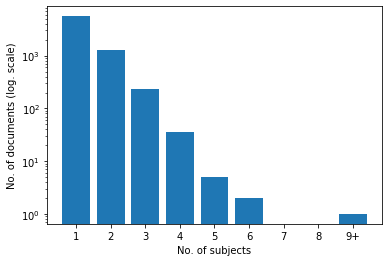
\includegraphics[width=\textwidth]{figures/evaluation/subjects_per_doc.png}
    \caption{Handwritten subjects.}
    \label{fig:subjects_per_doc}
  \end{subfigure}
  \hfill
  \begin{subfigure}[t]{0.45\textwidth}
    \centering
    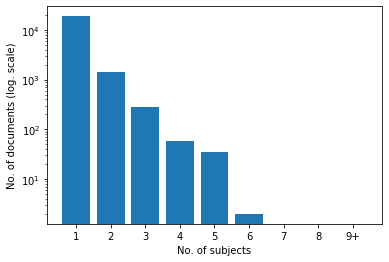
\includegraphics[width=\textwidth]{figures/evaluation/ddc_per_doc.png}
    \caption{DDC subjects.}
    \label{fig:ddc_per_doc}
  \end{subfigure}
  \caption{Number of subjects (handwritten or DDC) assigned to each document.}
\end{figure}

\subsubsection{DDC subjects} \label{eval_ddc}

Mapping \acrshort{ddc} subjects to \acrshort{mag} subjects was more complicated than with the handwritten subjects of the repositories, as they are numbers and cannot be mapped through a basic string matching procedure. In section \ref{eval_ddc_map}, we show how we have manually mapped \acrshort{ddc} number to the \acrshort{mag} fields of study. We could find \acrshort{ddc} numbers for all fields except for \textit{Materials science}, \textit{Business} and \textit{Environmental science}.

We present the resulting evaluation set in section \ref{eval_ddc_results}. It comprises over 22,000 assignments, including 70 \% of all documents, making this evaluation set the largest of the three. Depositonce is the repository that is worse represented by this set, with a coverage of 31 \%.

\paragraph{Mapping procedure} \mbox{} \label{eval_ddc_map}

We have manually mapped \acrshort{ddc} subclasses to the \acrshort{mag} fields of study. This is straight forward, as most of the fields of study have equivalent \acrshort{ddc} subclasses. For example, \textit{Biology} is a field in \acrshort{mag} and also a \acrshort{ddc} subclass, with the number $570$. The same is true for almost all fields, except for \textit{Materials Science}, \textit{Business} and \textit{Environmental Science}. \textit{History} and \textit{Philosophy}, on the other hand, have multiple \acrshort{ddc} subclasses, as their broad subjects are divided into more concrete fields. For example, \textit{History} has one subclass per continent, as well as others. The whole mapping of \acrshort{ddc} subclasses to \acrshort{mag} fields is depicted in table \ref{tab:ddc_fields}.

\begin{table}[]
    \centering
    \begin{tabular}{|c|c|}
        \hline
        \textbf{MAG field} & \textbf{DDC subclasses} \\ \hline\hline
        Medicine & 610 \\ \hline
        Chemistry & 540 \\ \hline
        Biology & 570 \\ \hline
        Computer Science & 000 \\ \hline
        Materials Science &  \\ \hline
        Engineering & 620 \\ \hline
        Psychology & 150 \\ \hline
        Physics & 530 \\ \hline
        Political Science & 320 \\ \hline
        Mathematics & 510 \\ \hline
        Business &  \\ \hline
        Sociology & 300 \\ \hline
        Geography & 910 \\ \hline
        Art & 700 \\ \hline
        Environmental Science &  \\ \hline
        Economics & 330 \\ \hline
        Geology & 550 \\ \hline
        History & 900, 910, 940-990 \\ \hline
        Philosophy & 100, 120, 140-190 \\ \hline
    \end{tabular}
    \caption{Manual mapping of DDC subclasses to MAG fields of study.}
    \label{tab:ddc_fields}
\end{table}

All \acrshort{ddc} subclasses and more specific subjects under each of the subclasses shown in table \ref{tab:ddc_fields} are also included in our evaluation set. For instance, the \acrshort{ddc} subject \textit{Philosophy of Germany and Austria}, number $193$, is a descendant of the \acrshort{ddc} subclass \textit{Modern western philosophy}, which has the number $190$. We therefore include all \acrshort{ddc} numbers that start with $19$ (or any other number of table \ref{tab:ddc_fields}) in our evaluation set.

\paragraph{Evaluation set} \mbox{} \label{eval_ddc_results}

Applying the mapping procedure explained above yields an evaluation set that comprises 22,915 assignments. As can be seen in figure \ref{fig:eval_ddc_fields}, \textit{Medicine} is by far the most popular field, with 3,611 assignments. \textit{Physics}, \textit{Biology} and \textit{Economics} also have more than 2,000 assignments. In total, this set comprises 20,636 documents, which amount to 70 \% of the 29,399 documents in our dataset. 18,865 of them have only one \acrshort{ddc} subject assigned to them, whereas two documents have six \acrshort{ddc} subjects. The number of \acrshort{ddc} subjects per document is depicted in figure \ref{fig:eval_ddc_fields}. On average, documents are assigned 1.1 \acrshort{ddc} subjects.

Regarding the repositories, depositonce is the repository with the least assignments. 2,333 of its documents have been assigned \acrshort{ddc} subjects, which accounts for 31 \% of its documents. Edoc and refubium, on the other hand, have \acrshort{ddc} subjects assigned to 77 \% and 86 \% of their documents, respectively. Figure \ref{fig:docs_per_ddc} shows how frequently \acrshort{ddc} subjects are assigned to documents. 49 \% of the \acrshort{ddc} subjects are assigned to at least nine documents. On the other hand, 32 \% are assigned to only one document. On average, \acrshort{ddc} subjects are assigned to 129 documents.

In total, there are 177 distinct \acrshort{ddc} subjects. 28 of them are classes or subclasses, i.e. their numbers end in $0$, and the rest are more specific. The classes and subclasses, having larger scopes, are assigned to 623 documents on average, whereas the rest of the \acrshort{ddc} subjects are assigned to 37 documents, on average. \textit{History} has by far the most distinct \acrshort{ddc} subjects, with 41, followed by \textit{Philosophy}, with 18. \textit{Art} is the field with the least \acrshort{ddc} subjects, with six (ignoring the three fields that could not be mapped to any \acrshort{ddc} subclasses).

\subsubsection{Venues} \label{eval_venues}

Venues are also good descriptors of the topics handled by a publication. They are similar to \acrshort{ddc} subjects in their scope; they can't be used to evaluate the most specific subjects, but can be useful to assess if the indexing procedures are guessing the right \acrshort{mag} field of study of each document.

Mapping venues to fields must also be done manually. We perform a similar procedure as was done for the \acrshort{ddc} subjects in the previous section. We therefore also divide this section in two parts: how venues were mapped to subjects, and then the resulting evaluation set.

\paragraph{Mapping procedure} \mbox{}

As mentioned in section \ref{repo_analysis_venues}, there are 4,418 distinct venues, 2,867 of which (65 \%) are only assigned to one publication. We therefore filter out the most popular ones, i.e. those that appear in at least ten documents. Recall that we also consider advisors and referees, so that theses can be grouped as well. There are 70 venues, 13 advisors and 70 referees with more than ten documents. From now on, we also refer to advisors and referees when we mention venues, as that is their role in this section.

The venues with more than 10 documents cover only the most popular fields. We therefore had to look online for professors of disciplines that were not present in this list of venues, such as \textit{Geology}, \textit{Sociology}, or \textit{Business}. In the end, we have manually assigned 132 venues to the \acrshort{mag} fields. \textit{Art} is the only field for which we could not find any venue in the repositories. The mapping of venues to fields can be found in Appendix \ref{appendix_venue_map}. There you can also find how many documents belong to each venue.

Although it is not relevant for this evaluation set, it is worth noting the presence of duplicates in the lists of referees and advisors. While mapping professors to \acrshort{mag} fields, we sometimes found the same professor under different names. For example, Prof. Dr. Charlotte M. Krawzcyk appears in the repositories under six different names, and Prof. Dr. Michael C. Burda, under five different names. This issue was already mentioned in section \ref{repo_analysis_contributors}.

\paragraph{Evaluation set} \mbox{}

Once we have assigned the venues to the \acrshort{mag} fields, we can use this mapping to assign documents to fields, just as we did to create the \acrshort{ddc} evaluation set. Figure \ref{fig:eval_venue_fields} shows the distribution of documents in this evaluation set per field. As happened with the evaluation sets derived from the subjects, the natural sciences are better represented than the social sciences. \textit{Chemistry} has the most documents, with 499, followed by \textit{Computer Science} and \textit{Physics}, with 449 and 399 documents, respectively. \textit{Art}, \textit{Political science} and \textit{Geology} are the worst represented fields, with 0, 8 and 21 documents, respectively.

An important difference between this evaluation set and the other two is how well represented \textit{Environmental science} is. In the evaluation set derived from the handwritten subjects, this field had the least documents, with 41 documents, and in the \acrshort{ddc} evaluation set it had none. Here it has 291 documents.

\begin{figure}
    \centering
    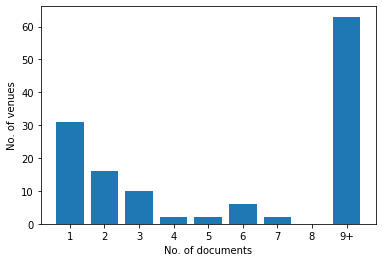
\includegraphics[width=.7\textwidth]{figures/evaluation/docs_per_venue.png}
    \caption{Number of documents per venue}
    \label{fig:docs_per_venue}
\end{figure}

Figure \ref{fig:docs_per_venue} shows the number of documents per venue. Almost half (48 \%) of the venues in our set are assigned to at least nine documents, whereas 23 \% are assigned to only one. These venues that are assigned to only one document are the professors of fields for which there weren't any popular venues in the repositories. Documents are usually only assigned one venue. This is always the case for publications, which are only be published in one place, but not necessarily for theses, which can have multiple advisors or referees. In our evaluation set, only 2 \% of the documents have more than one venue, and never more than two.

\subsubsection{Summary of the evaluation sets} \label{eval_datasets_summary}

After presenting each evaluation set individually, we now look at them as a whole, focusing on their coverage of repositories (table \ref{tab:eval_repo_coverage}) and fields (figure \ref{fig:eval_field_distribution}). We refer to them as the handwritten set, the \acrshort{ddc} set and the venue set for brevity.

The \acrshort{ddc} set covers by far the most documents of all repositories. As shown in table \ref{tab:eval_repo_coverage}, it covers 70 \% of the documents in all three repositories. depositonce is the repository worst represented in this evaluation set, with only 31 \% coverage. The handwritten set covers more than twice as many documents as the venue set. Contrary to the \acrshort{ddc} set, both these sets cover more of depositonce than of any other repository. This is remarkable given that depositonce is a much smaller repository than refubium.

\begin{table}[]
    \centering
    \begin{tabular}{|c|c|c|c|c|}
        \hline
        \textbf{Evaluation set} & \textbf{total} & \textbf{depositonce} & \textbf{edoc} & \textbf{refubium} \\ \hline \hline
        \textbf{Handwritten} & 24 \% & 29 \% & 23 \% & 22 \% \\ \hline
        \textbf{DDC} & 70 \% & 31 \% & 78 \% & 86 \% \\ \hline
        \textbf{Venues} & 11 \% & 16 \% & 14 \% & 8 \% \\ \hline
    \end{tabular}
    \caption{Repository coverage of the evaluation sets.}
    \label{tab:eval_repo_coverage}
\end{table}

Figure \ref{fig:eval_field_distribution} compares the coverage of the \acrshort{mag} fields by the evaluation sets, in percentages. The field percentages of an evaluation set results add up to 100 \%. The \acrshort{ddc} evaluation set is the most polarized of all. 18 \% of its documents belong to the field of \textit{Medicine}, and the fields \textit{Biology}, \textit{Physics} and \textit{Economics} each represent 13 \% of the evaluation set. Thus, 57 \% of the documents of the \acrshort{ddc} evaluation set belong to only four fields, out of 19.

The popularity of \textit{Medicine} in the \acrshort{ddc} set results of its large coverage of refubium (86 \%), which is the largest repository of the three and includes documents from Charité, the Medical University of Berlin. \textit{Economics} is a popular field both in \textit{refubium} and \textit{edoc}, as was discussed in chapter \ref{repo_analysis_subjects}. Furthermore, the \acrshort{ddc} evaluation set does not have any documents of the fields \textit{Materials science}, \textit{Business} and \textit{Environmental science}, as well as barely any belonging to \textit{Art} or \textit{Geography}. Therefore, there are three empty fields and two that are barely represented in this set.

The handwritten set is the most evenly distributed set regarding fields, and is the only one that covers all fields. The fields that stand out the most are \textit{Biology}, which accounts for 12 \% of the documents, followed by \textit{Medicine} and \textit{Physics}, both with 8 \% of the documents. Its worst represented fields are \textit{Business}, \textit{Environmental Science} and \textit{Art}, which are also among the least represented fields of the \acrshort{ddc} set.

The venue set is dominated by depositonce and edoc, which almost double refubium regarding repository coverage. This explains the two most popular fields, which differ from those in the other evaluation sets, as they do not appear often in refubium: \textit{Chemistry} accounts for 13 \% of the documents, and \textit{Computer science}, for 12 \%. On the other hand, this set doesn't have any documents for \textit{Art} and barely any for \textit{Philosophy}, \textit{History}, \textit{Geology}, \textit{Sociology}, \textit{Business} and \textit{Political Science}. These seven fields account for only 4.5 \% of the documents of this evaluation set.

\begin{figure}
    \centering
    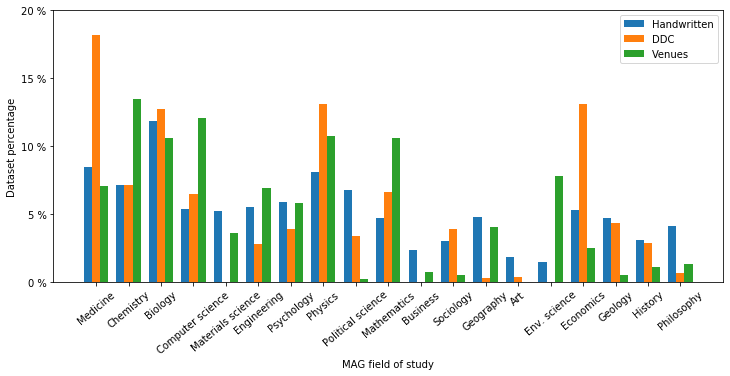
\includegraphics[width=\textwidth]{figures/evaluation/eval_field_distribution.png}
    \caption{Distribution of the evaluation set among the MAG fields of study.}
    \label{fig:eval_field_distribution}
\end{figure}

The natural sciences dominate all evaluation sets. It can be clearly seen in figure \ref{fig:eval_field_distribution}, where the bars to the left are much higher than those to the right. \textit{Medicine}, \textit{Biology} and \textit{Physics} appear more than 1,200 times in all three evaluation sets, mainly due to the \acrshort{ddc} evaluation set, which covers far more documents than the other two sets. On the other end of the spectrum, \textit{Art} and \textit{Business} are the only fields with less than 100 appearances in the evaluation sets. However, the average number of appearances per field exceeds 540 documents.